\chapter{Эксперименты} \label{chapt3}

Описанные в главах \ref{chapt1} и \ref{chapt2} алгоритмы имеют значительное
количество параметров. Для подбора их оптимальной комбинации, фактически,
необходимо решить задачу многомерной оптимизации в достаточно большом
пространстве. Очевидно, что в данном случае невозможно решить эту задачу
аналитически. Также невозможно перебрать все возможные комбинации параметров
ввиду слишком большого их числа. Однако во многих случаях можно определить
разумный диапазон возможных значений параметра и исследовать изменение качества
распознавания аккордов в зависимости от значений данного параметра в указанном
диапазоне.

Применение методов вычисления классификации векторов признаков, основывающихся
на машинном обучении, не позволяет целиком избавиться от ручного подбора
параметров. Во-первых, эти алгоритмы могут иметь метапараметры, не изменяемые в
процессе обучения (например, количество нейронов в $j$-м слое нейронной сети).
Во-вторых, параметры имеются также на этапах подготовки входных данных и
интерпретации результата.

Поскольку все эксперименты проводились на описанной в разделе \ref{ssectT_coll}
коллекции из 312 музыкальных звукозаписей, найденные значения параметров будут
оптимальными только для этой коллекции. Способствовать преодолению этой проблемы
могли бы достаточно большие коллекции аннотированных композиций, не существующие
на данный момент.

Все эксперименты можно разделить на 4 группы. В разделе \ref{sect3_spectcalc}
рассматривается этап предварительной обработки звукозаписи и получения
спектрограммы. В разделе \ref{sect3_specttrans} исследуется влияние различных
преобразований спектрограммы на качество распознавания аккордов. Эксперименты
в разделе \ref{sect3_nn} направлены на отыскание наилучших параметров нейронной
сети, используемой для получения признаков. Преобразования над
последовательностями векторов признаков и распознанных аккордов и параметры
выбранного метода классификации анализируются в разделе \ref{sect3_class}. В
разделе \ref{sect3_time} сравниваются скорости работы реализованных алгоритмов.

\section{Оценка качества распознавания аккордов} \label{sect3_eval}

Поскольку алгоритмы распознавания аккордов предназначаются для обработки
музыкальных звукозаписей, необходимо оценивать качество их работы на реальных
звукозаписях, а не на искусственно сгенерированных примерах. Чтобы звукозапись
можно было использовать для оценки, требуется вручную решить задачу
распознавания последовательности аккордов, то есть для каждого момента времени
$t \in [t_{start}, t_{end}]$ указать аккорд $y \in \overline{Y}$, звучащий в
этот момент. При этом набор $\overline{Y}$ включает в себя все возможные в
музыке сочетания нот и отдельные ноты. Также требуется с высокой точностью
указать моменты начала и конца звучания аккордов. Всё это делает задачу
подготовки тестовых коллекций очень трудоёмкой.

Для хранения этой информации используют особым образом отформатированные
текстовые файлы, называемые файлами разметки или файлами текстовых аннотаций.
Ниже приведён пример такого файла:
\begin{lstlisting}
0.000	0.848	N
0.848	1.625	A:min
1.625	3.017	G:maj
3.017	3.895	F:maj
...
\end{lstlisting}
Первый и второй столбцы содержат время начала и конца звучания аккорда
соответственно, в третьем столбце записывается название аккорда. 

\subsection{Коллекции текстовых аннотаций} \label{ssectT_coll}

На текущий момент существует 5 коллекций текстовых аннотаций для популярной
музыки разных исполнителей:
\begin{itemize}
  \item \emph{Isophonics} \cite{MauchOmp2009}. Текстовые аннотации для 180
  композиций (12 альбомов) \textit{The Beatles}, 20 композиций \textit{Queen}
  (с альбома \textit{Greatest Hits}), 18 композиций \textit{Zweieck} (с альбома
  \textit{Zweilicht}). Наиболее часто используется для исследований, несколько
  раз использовалась для ежегодных соревнований MIREX Audio Chord Estimation.
  
  \item \emph{RWC Pop Music} \cite{Goto2002}. Текстовые аннотации для 100
  композиций японской и западной популярной музыки.
  
  \item \emph{Billboard} \cite{Burgoyne2011}. Текстовые аннотации для 197
  композиций из американского чарта \textit{Billboard 100} за промежуток с 1958
  по 1991 год. Использовалась в соревновании MIREX Audio Chord Estimation в 2012
  году.
  
  \item \emph{uspop2002} \cite{Berenzweig2004}. Текстовые аннотации для 195
  композиций американской популярной музыки.
  
  \item \emph{Robbie Williams annotations}. Текстовые аннтоации для 65
  композиций \textit{Robbie Williams} (первые 5 альбомов).
\end{itemize}

Поскольку в аннотациях указывается точное время, важно при анализе использовать
точно те же версии звукозаписей, которые были использованы при подготовке
аннотаций. Это затрудняет использование некоторых коллекций. Для тестирования
алгоритмов в рамках данной работы использовались коллекции \emph{Isophonics} и
\emph{RWC Pop Music}.

\subsection{Сопоставление последовательностей аккордов}

Вопросом оценки того, насколько одна последовательность аккордов (определённая
автоматически) соответствует другой (правильной, определённой человеком),
занимались Харте \cite{Harte2010} и Пауэлс и Питерс \cite{Pauwels2013}.
Последние предлагают следующую конструкцию для определения схожести двух
последовательностей аккордов.

\begin{figure} [h] 
  \center
  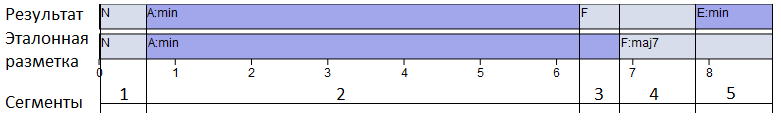
\includegraphics [scale=0.80] {EvaluationSegments}
  \caption{Сопоставление последовательностей аккордов.}
  \label{img:evaluation_segments}  
\end{figure}

Пусть заданы 2 последовательности аккордов: правильная и определённая при помощи
алгоритма. Объединим множества границ аккордов из обоих последовательностей в
одно множество. Используя эти границы, разделим исходную композицию на
сегменты (как на рисунке \ref{img:evaluation_segments}), на каждом из которых
однозначно заданы правильный аккорд $c_{ref}$ и определённый автоматически
$c_{est}$. Пусть также $c_{ref} \in C_{REF}$ -- множество всех аккордов,
встречающихся в аннотациях, а $c_{est} \in C_{EST}$ -- множество всех аккордов,
которые могут быть результатом распознавания при помощи данного алгоритма.

Практически всегда $C_{EST} \subset C_{REF}$, поэтому возникает вопрос о том,
как сопоставлять фрагменты, на которых $c_{ref} \not \in C_{EST}$. Такие
фрагменты можно либо отбрасывать, либо задать сюръективное отображение
$\mathcal{M}: C_{MI} \to C_{MO}$, которое <<сложным>> аккордам из множества
$C_{MI}$ будет сопоставлять <<простые>> аккорды из множества $C_{MO}$. Нужно
выбрать эти множества и отображение $\mathcal{M}$ таким образом, чтобы $C_{EST}
\subset C_{MI}$. Сравниваться при этом будут аккорды $\mathcal{M}(c_{ref})$ и
$\mathcal{M}(c_{est})$. Сегменты, на которых $c_{ref} \not \in C_{MI}$,
отбрасываются. Примером отображения $\mathcal{M}$ может служить отображение,
которое всем аккордам, состоящим из мажорного трезвучия и более высоких ступеней
(например, доминантсептаккорд, нонаккорды и другие) сопоставляет мажорный
аккорд, соответствующий этому трезвучию.

Если необходимо оценить качество распознавания аккордов определенного типа
(например, только трезвучий или только мажорных аккордов), можно ввести
дополнительные множества $C_{LI}$ и $C_{LO}$, ограничивающие соответственно
множества $C_{MI}$ и $C_{MO}$. Тогда аккорды $(c_{ref}, c_{est})$ сравниваются
(не отбрасываются), только если $c_{ref} \in C_{LI} \cap C_{MI}$ и
$\mathcal{M}(c_{ref}) \in \mathcal{M}(C_{LI} \cap C_{MI}) \cap C_{LO}$.

Пусть $\mathcal{S}:C_{SR} \times C_{SE} \to \mathbb{R}^+$ -- функция оценки,
причем $\mathcal{M}(C_{LI} \cap C_{MI}) \cap C_{LO} \subset C_{SR}$ и $C_{MO}
\subset C_{SE}$. Эта функция сопоставляет паре аккордов $\mathcal{M}(c_{ref})$ и
$\mathcal{M}(c_{est})$ неотрицательное действительное число, которое выражает
сходство этих аккордов между собой. Например, можно определить функцию
$\mathcal{S}$ как равную 1 в случае, когда аккорды совпадают, и 0 иначе.

Как видно из \cite{Pauwels2013}, полученные цифры сильно различаются в
зависимости от выбора отображения $\mathcal{M}$ и функции оценки $\mathcal{S}$,
и даже в зависимости от некоторых мелких деталей, таких как способ
синтаксического разбора названий аккордов. Не всегда в статьях корректно
указываются использованные метрики, что делает затруднительным непосредственное
сравнение оценок качества распознавания из статей друг с другом. В этом состоит
главная ценность соревнования MIREX Audio Chord Estimation, где гарантированно
используются одни и те же коллекции и метрики для оценки всех алгоритмов.

В экспериментах в рамках данной работы будем использовать метрику ``Mirex2010''
из \cite{Pauwels2013}. В ней не используется отображение $\mathcal{M}$, а
функция оценки $\mathcal{S}$ строится следующим образом. Сначала $c_{ref}$ и
$c_{est}$ преобразуются в множества тональных классов, для которых находится
пересечение. Обозначим количество элементов в пересечении за $u$.
$\mathcal{S}=1$ в случаях:
\begin{itemize}
  \item $c_{ref}$ является уменьшенным или увеличенным аккордом и $u \geq 2$;
  \item $c_{ref}$ и $c_{est}$ являются символами отсутствия аккорда;
  \item $u \geq 3$.
\end{itemize}
В остальных случаях $\mathcal{S}=0$, то есть $\mathcal{S}:C_{SR} \times C_{SE}
\to \{0, 1\}$. 

Отметим, что при использовании этой метрики ни один сегмент не
отбрасывается. Её выбор является в достаточной степени произвольным и связан
исключительно с тем фактом, что именно она использовалась в соревновании MIREX
Audio Chord Estimation в 2010, 2011 и 2012 годах.

Пусть $\ell_1, \ell_2, \ldots, \ell_{N_{segm}}$ -- длины всех сегментов в
пределах одной композиции, а $s_1, s_2, \ldots, s_{N_{segm}}$ -- соответствующие
значения метрики. Тогда \emph{коэффициент перекрытия (overlap ratio, OR)} для
данной композции определяется как
\begin{equation} \label{eq:or}
OR = \frac{\sum_{i=1}^{N_{segm}} s_i \ell_i}{\sum_{i=1}^{N_{segm}} \ell_i}
\end{equation}
При этом неважно, были ли ceгменты взяты из одной и той же композиции или из
нескольких разных. Но для того, чтобы иметь возможность определить
статистически значимые различия между системами, в экспериментах будем
определять коэффициент перекрытия отдельно для каждой композиции.

Для примера, на рисунке \ref{img:evaluation_segments} $s_1 = s_2 = s_4 = 1$,
$s_3 = s_5 = 0$. На сегментах 1 и 2 аккорды совпадают, на сегменте 4 аккорды
F:maj и F:maj7 имеют 3 общих ступени F, A, C.

Пусть коллекция содержит $N_{tracks}$ композиций, для каждой из которых
вычислен коэффициент перекрытия $OR_k$. Обозначим за $L_i =
\sum_{i=j}^{N_{segm}} \ell_j$ длину $i$-й композиции. Тогда совокупная метрика
для коллекции, называемая \emph{взвешенным средним коэффициентом перекрытия
(weighted average overlap ratio, WAOR)}, вычисляется следующим образом:
\begin{equation} \label{eq:waor}
WAOR = \frac{\sum_{i=1}^{N_{tracks}} OR_i \cdot L_i}{\sum_{i=1}^{N_{tracks}}
L_i}
\end{equation}
Такой же способ усреднения применяется в соревнованиях MIREX Audio Chord
Estimation.

\subsection{Сопоставление границ сегментов}

Метрика для сопоставления границ сегментов была введена Маухом в
\cite{MauchThesis2010}, но не получила широкого распространения. Она позволяет
оценить качество определения границ аккордов алгоритмом, игнорируя при этом сами
названия аккордов.

Пусть заданы 2 разбиения звукозаписи длины $L$ на сегменты $G^0 = (G_i^0)$ и $G
= (G_i)$. Направленное расхождение Хэмминга определяется как:
$$
h(G||G^0) = \sum_{i=1}^{N_G} \left( |G_i^0| - \underset{j}{\operatorname{max}}
|G_i^0 \cap G_j| \right)
$$
где $N_G$ -- количество сегментов в разбиении $G$, а $| \cdot |$ -- длина
сегмента. Оно определяет, насколько $G$ фрагментировано по отношению к $G^0$.
Тогда \emph{сегментация} $H(G, G^0)$ определяется как
$$H(G, G^0) = 1 - \frac{1}{L} max\{ h(G||G^0), h(G^0||G) \} \in [0,1]$$

\subsection{Статистическая значимость}

При сравнении нескольких вариантов алгоритма помимо средних значений метрик
качества необходимо понять, действительно ли между этими вариантами имеются
статистически значимые различия. Для проверки этого предположения будем
использовать непараметрический критерий Фридмана. Он позволяет проверять
гипотезы о различии более двух зависимых выборок. В отличие от дисперсионного
анализа (ANOVA), критерий Фридмана не требует предположений о нормальности
распределения значений метрик для разных композиций, а также одинаковых
дисперсий этих распределений для разных вариантов алгоритма (как отмечается в
\cite{Mauch2010}, эти предположения не является верными в данном случае).

Однако, если в соответствии с критерием Фридмана удаётся отвергнуть нулевую
гипотезу (об отсутствии различий между разными методами), необходимо выяснить,
для каких пар методов имеется статистически значимая разница в качестве
распознавания аккордов. Для этого вычисляется среднее Тьюки (Tukey's honestly
significant difference). В отличие от T-теста, при его допускаются множественные
попарные сравнения. Этот метод используется для сравнения качества работы разных
алгоритмов в рамках всех соревнований MIREX \cite{Downie2008}.

\section{Вычисление спектрограммы} \label{sect3_spectcalc}

На данном этапе необходимо выбрать наилучшие из доступных алгоритмов для
определения ритма и определения частоты настройки. Кроме того, необходимо
определить наилучшие значения для параметров преобразования постоянного
качества: разрешение по частоте $N_0$ (количество компонент, приходящихся на
октаву) и количество октав $N / N_0$, а также для количества вставляемых
промежуточных столбцов спектрограммы $T$ и размера окна при сглаживании $w$.

\subsection{Определение ритма} \label{ssect3_beattrack}

Были рассмотрены 3 алгоритма, позволяющие определить моменты начала метрических
долей в звукозаписи: \emph{BeatRoot} \cite{Dixon2007}, \emph{Beat tracker} от
Дэвиса \cite{Davies2007} (\emph{DBT}) из набора плагинов \emph{Queen Mary Vamp
plugins}\footnote{\url{http://www.isophonics.net/QMVampPlugins}} для системы
извлечения музыкальной информации из музыкальных файлов
\emph{Vamp}\footnote{\url{http://www.vamp-plugins.org/}} и плагина \emph{INESC
Porto Beat Tracking plugin} \cite{Oliveira2012} (\emph{IBT}) для этой же
системы. Выбор алгоритмов обусловлен наличием свободно доступной реализации.
\emph{BeatRoot} дополнительно потребовал небольшого вмешательства в исходный
код для уменьшения потребления вычислительных ресурсов. Кроме того, на 6
композициях из анализруемого набора этот алгоритм не смог определить ритм,
поэтому для этих композиций использовались значения, полученные при помощи DBT.

\begin{table} [htbp]
  \centering
  \parbox{15cm}{\caption{Влияние алгоритма определения ритма на
  качество распознавания аккордов} \label{TBT}}
%  \begin{center}
  \begin{tabular}{|l|l|l|l|}
  \hline
  Алгоритм & WAOR & Сегментация \\
  \hline
  BeatRoot + DBT & 0.7516 & 0.7907 \\
  DBT & 0.7317 & 0.7659 \\
  IBT & 0.7189 & 0.7425 \\
  \hline
  \end{tabular}
%  \end{center}
\end{table}

Наилучшие полученные для данных алгоритмов результаты показаны в таблице
\ref{TBT}. \emph{BeatRoot} показал наилучший результат, статистически значимо
превосходящий результаты, полученные с использованием алгоритмов \emph{IBT} и
\emph{DBT}. Это достаточно удивительно, поскольку первая версия алгоритма
\emph{BeatRoot} была представлена ещё в 2001 году, а в данной работе
использовалась его исправленная версия от 2007 года. При этом \emph{DBT} был
представлен в 2007 году, а \emph{IBT}, схожий по принципу работы с
\emph{BeatRoot}, -- в 2012 году.

\subsection{Определение частоты настройки} \label{ssec3_tunfreq}

Были проведены эксперименты по распознаванию аккордов с использованием
описанного в разделе \ref{ssect1_f0} алгоритма для вычисления частоты настройки
со следующими значениями параметров:
\begin{itemize}
  \item $f_{min} = 220$ Гц, $N_0 = 12 \cdot 20 = 240$ компонент на октаву;
  \item $f_{min} = 220$ Гц, $N_0 = 12 \cdot 10 = 120$ компонент на октаву;
  \item $f_{min} = 440$ Гц, $N_0 = 12 \cdot 20 = 240$ компонент на октаву.
\end{itemize}
Охват во всех случаях составлял 4 октавы. Также для сравнения были проведены
эксперименты без коррекции частоты настройки и с использованием алгоритма,
описанного Маухом в \cite{MauchThesis2010}, раздел 3.1.3 и реализованного в виде
плагина для системы \emph{Vamp}.

\begin{table} [htbp]
  \centering
  \parbox{15cm}{\caption{Влияние алгоритма определения частоты настройки на
  качество распознавания аккордов} \label{TTunFreq}}
  \begin{tabular}{|l|l|l|l|}
  \hline
  Алгоритм & WAOR & Сегментация \\
  \hline
  $f_{min} = 220$ Гц, $N_0 = 120$ & 0.7516 & 0.7892 \\
  $f_{min} = 220$ Гц, $N_0 = 240$ & 0.7516 & 0.7907 \\
  $f_{min} = 440$ Гц, $N_0 = 240$ & 0.7512 & 0.7899 \\
  Маух \cite{MauchThesis2010} & 0.7477 & 0.7888 \\
  -- & 0.7429 & 0.7854 \\
  \hline
  \end{tabular}
\end{table}

Результаты экспериментов приведены в таблице \ref{TTunFreq}. Как видно,
определение частоты настройки приводит к улучшению качества распознавания
аккордов, причем при использовании любого из перечисленных алгоритмов это
улучшение статистически значимо. Использование любого из описанных вариантов
алгоритма из раздела \ref{ssect1_f0} также приводит к статистически значимому
улучшению по сравнению с алгоритмом Мауха, но за счёт большего времени работы. В
то же время между собой эти 3 варианта отличаются незначительно.

\subsection{Разрешение по времени и по частоте, сглаживание}

Вставка между каждыми двумя соседними моментами начала метрических долей
$T-1$ промежуточных значений позволяет повысить разрешение спектрограммы по
времени. Затем, после применения скользящего медианного фильтра с размером окна
$w$ и прореживания в $T$ раз, спектрограмма содержит ровно 1 столбец на каждую
метрическую долю. Ясно, что при больших значениях $T$ имеет смысл выбирать
больше значения $w$ и наоборот. В таблице \ref{TTw} приведены значения для
некоторых комбинаций $T$ и $w$.

\begin{table} [htbp]
  \centering
  \parbox{15cm}{\caption{Влияние параметров $T$ и $w$ на качество распознавания
  аккордов} \label{TTw}}
  \begin{tabular}{|l|l|l|}
  \hline
  Значения параметров & WAOR & Сегментация \\
  \hline
  $T = 2$, $w = 1$ & 0.6780 & 0.7561 \\
  $T = 2$, $w = 3$ & 0.7368 & 0.7830 \\
  $T = 2$, $w = 5$ & 0.7278 & 0.7721 \\
  \hline
  $T = 4$, $w = 5$ & 0.7467 & 0.7886 \\
  $T = 4$, $w = 7$ & 0.7496 & 0.7884 \\
  $T = 4$, $w = 9$ & 0.7451 & 0.7827 \\
  \hline
  $T = 8$, $w = 13$ & 0.7504 & 0.7910 \\
  $T = 8$, $w = 15$ & 0.7516 & 0.7907 \\
  $T = 8$, $w = 17$ & 0.7494 & 0.7863 \\
  \hline
  \end{tabular}
\end{table}

При $T=2$ качество распознавания аккордов существенно хуже для случая $w=1$, что
фактически соответствует отказу от добавления промежуточных значений и
последующих сглаживания и прореживания. Статистически значимых отличий между
вариантами $w=3$ и $w=5$ нет.

При $T=4$ влияние параметра $w$ уже не столь существенно. Наилучший результат
получен при $w=7$, и он статистически значимо превосходит результаты, полученные
при $w=5$ и $w=9$ (разница между которыми, в свою очередь, не является
значимой).

При $T=8$ только разница между вариантами $w=15$ и $w=17$ оказалась
статистически значимой. При этом в абсолютных значениях различия ещё меньше, чем
для $T=4$.

Отдельно было проведено сравнение наилучших вариантов для каждого значения $T$.
Между вариантами $T=4, w=7$ и $T=8, w=15$ нет статистически значимой разницы в
качестве распознавания аккордов; разница в абсолютных значениях метрик также
незначительна. При $T=2, w=3$ был получен существенно худший результат.

Интересно, что наилучшие резултаты достигаются при $w = 2T-1$, что для каждого
момента времени исходной последовательности соответствует фильтрации по
значениям спектра, вычисленным в этот момент и в $T-1$ добавленных промежуточных
точках справа и слева. Из этого эксперимента видно, что увеличение разрешения по
времени для последовательности моментов начала метрических долей по крайней мере
в 4 раза приводит к существенному улучшению качества распознавания аккордов.

\begin{table} [htbp]
  \centering
  \parbox{15cm}{\caption{Влияние параметра $N_0$ на качество распознавания
  аккордов} \label{TN0}}
  \begin{tabular}{|l|l|l|l|}
  \hline
  Значения $N_0$ & WAOR & Сегментация \\
  \hline
  $N_0 = 12$ & 0.6257 & 0.7743 \\
  $N_0 = 36$ & 0.7518 & 0.7951 \\
  $N_0 = 60$ & 0.7516 & 0.7907 \\
  \hline
  \end{tabular}
\end{table}

В таблице \ref{TN0} приведены результаты, полученные при разных значениях
количества компонент преобразования постоянного качества, приходящихся на одну
октаву. Очевидно, что при наличии как минимум 36 компонент на октаву (3
компоненты на ноту) качество распознавания аккордов существенно повышается.
Различия между $N_0=36$ и $N_0=60$ не являются статистически значимыми. Однако
при $N_0=60$ требуется вычислить в 1.8 раз больше значений для компонент
преобразования постоянного качества, а также в дальнейшем многократно вычислять
дискретное косинусное преобразование для большего набора значений.

% Основные вопросы относительно выбора параметров, возникающие на этом этапе:
% \begin{enumerate}
%   \item действительно ли определение частоты настройки музыкальных инструментов
%   повышает качество распознавания аккордов;
%   \item каковы оптимальные параметры алгоритма определения частоты настройки;
%   \item действительно ли определение ритма повышает качество распознавания
%   аккордов;
%   \item есть ли разница между библиотеками \emph{Beatroot} \cite{Dixon2007} и
%   \emph{Beat tracker} \cite{Davies2007} из набора \emph{Queen Mary Vamp
%   plugins};
%   \item возможно ли добиться при помощи быстрого преобразования Фурье и
%   последующего отображения полученного спектра на частоты звукоряда по формуле
%   \ref{fft_wrap} такого же качества распознавания, как при использовании
%   преобразования постоянного качества;
%   \item каковы оптимальные значения для разрешения по частоте $N_0$ (количество
%   компонент, приходящихся на октаву) и количества октав $N / N_0$ в
%   преобразовании постоянного качества;
%   \item каковы оптимальные значения для количества вставляемых промежуточных
%   столбцов спектрограммы $T-1$ и размера окна при сглаживании $w$.
% \end{enumerate}

% \begin{table} [htbp]
%   \centering
%   \parbox{15cm}{\caption{Название таблицы}\label{Ts0Sib}}
% %  \begin{center}
%   \begin{tabular}{| p{3cm} || p{3cm} | p{3cm} | p{4cm}l |}
%   \hline
%   \hline
%   Месяц   & \centering $T_{min}$, К & \centering $T_{max}$, К &\centering  $(T_{max} - T_{min})$, К & \\
%   \hline
%   Декабрь &\centering  253.575   &\centering  257.778    &\centering      4.203  &   \\
%   Январь  &\centering  262.431   &\centering  263.214    &\centering      0.783  &   \\
%   Февраль &\centering  261.184   &\centering  260.381    &\centering     $-$0.803  &   \\
%   \hline
%   \hline
%   \end{tabular}
% %  \end{center}
% \end{table}

\section{Преобразования спектрограммы} \label{sect3_specttrans}

Основные вопросы относительно выбора параметров, возникающие на этом этапе:
\begin{enumerate}
  \item действительно ли применение аналога фильтра Превитт повышает качество
  распознавания акокрдов;
  \item каково оптимальное значение для количества зануляемых первых
  коэффициентов дискретного косинусного преобразования $\xi$ при вычислении
  признаков CRP;
  \item действительно ли сглаживание с использованием матрицы самоподобия для
  столбцов спектрограммы лучше, чем с использованием такой матрицы для векторов
  признаков и без использования самоподобия вообще;
  \item каково оптимальное значение для доли сохраняемых в матрице самоподобия
  значений $\zeta$.
\end{enumerate}

\section{Нейронные сети} \label{sect3_nn}

Для описанного в главе \ref{chapt2} метода получения векторов признаков с
использованием нейронных сетей важными являются следующие вопросы:
\begin{enumerate}
  \item какое количество элементов во входном слое сети позволяет получить
  наилучшие векторы признаков;
  \item влияет ли предварительное применение логарифмического преобразования к
  спектрограмме на полученные векторы признаков;
  \item каковы оптимальное количество скрытых слоёв и их размеры в нейронной
  сети;
  \item действительно ли использование рекуррентных соединений повышает качество
  распознавания аккордов;
  \item каковы оптимальные значения для уровней шума при обучении очищающих
  автоассоциаторов;
  \item и др.
\end{enumerate}

Для проведения экспериментов тестовая коллекция из 318 композиций была случайным
образом поделена на 2 равные части, каждая из которых поочередно выступала в
качестве обучающей и тестовой выборки.

\section{Классификация векторов признаков} \label{sect3_class}

Для выбранного способа классификации векторов признаков необходимо определить
наилучшие значения следующих параметров:
\begin{enumerate}
  \item количество учитываемых при генерации шаблонов гармоник;
  \item степень убывания вклада гармоник в шаблон $s$.
\end{enumerate}
Помимо этого необходимо количественно оценить повышение качества распознавания
при использовании описанных в разделе \ref{ssect1_errcorr} эвристик.

\section{Быстродействие} \label{sect3_time}

\section{Выводы}

\begin{enumerate}
  \item TODO
\end{enumerate}

%\newpage
%============================================================================================================================

\clearpage